\documentclass[oneside,12pt,english]{book}
\usepackage{babel}
\usepackage[utf8]{inputenc}
\usepackage{color}
\definecolor{marron}{RGB}{60,30,10}
\definecolor{darkblue}{RGB}{0,0,80}
\definecolor{lightblue}{RGB}{80,80,80}
\definecolor{darkgreen}{RGB}{0,80,0}
\definecolor{darkgray}{RGB}{0,80,0}
\definecolor{darkred}{RGB}{80,0,0}
\definecolor{shadecolor}{rgb}{0.97,0.97,0.97}
\usepackage{graphicx}
\graphicspath{{img/}{02/media/}}
\usepackage{wallpaper}
\usepackage{wrapfig,booktabs}

\usepackage{fancyhdr}
\usepackage{lettrine}
\input Acorn.fd
\newcommand*\initfamily{\usefont{U}{Acorn}{xl}{n}}

\usepackage{geometry}
\geometry{
tmargin=5cm, 
bmargin=5.2cm, 
lmargin=5cm, 
rmargin=3cm,
headheight=1.5cm,
headsep=0.8cm,
footskip=0.5cm}


% \usepackage[full]{textcomp}
\renewcommand{\familydefault}{pplj} 
\usepackage[
final,
stretch=10,
protrusion=true,
tracking=true,
spacing=on,
kerning=on,
expansion=true]{microtype}

\setlength{\parskip}{1.3ex plus 0.2ex minus 0.2ex}


\usepackage{fourier-orns}

\newcommand{\ornamento}{\vspace{2em}\noindent \textcolor{darkgreen}{\hrulefill~ \raisebox{-2.5pt}[10pt][10pt]{\leafright \decofourleft \decothreeleft  \aldineright \decotwo \floweroneleft \decoone   \floweroneright \decotwo \aldineleft\decothreeright \decofourright \leafleft} ~  \hrulefill \\ \vspace{2em}}}
\newcommand{\ornpar}{\noindent \textcolor{darkgreen}{ \raisebox{-1.9pt}[10pt][10pt]{\leafright} \hrulefill \raisebox{-1.9pt}[10pt][10pt]{\leafright \decofourleft \decothreeleft  \aldineright \decotwo \floweroneleft \decoone}}}
\newcommand{\ornimpar}{\textcolor{darkgreen}{\raisebox{-1.9pt}[10pt][10pt]{\decoone \floweroneright \decotwo \aldineleft \decothreeright \decofourright \leafleft} \hrulefill \raisebox{-1.9pt}[10pt][10pt]{\leafleft}}}

\makeatletter
\def\headrule{{\color{darkgreen}\raisebox{-2.1pt}[10pt][10pt]{\leafright} \hrulefill \raisebox{-2.1pt}[10pt][10pt]{~~~\decofourleft \decotwo\decofourright~~~} \hrulefill \raisebox{-2.1pt}[10pt][10pt]{ \leafleft}}}
\makeatother

\fancyhf{}

\renewcommand{\chaptermark}[1]{\markboth{#1}{}}
\renewcommand{\sectionmark}[1]{\markright{#1}}

\newcommand{\estcab}[1]{\itshape\textcolor{marron}{\nouppercase #1}}

\fancyhead[LE]{\estcab{ESL in Action}}
\fancyhead[RE]{\estcab{The Old Woman Who Lived in a Shoe}}
% \fancyhead[CE,CO]{\estcab{\decoone}}
%\fancyhead[LO]{\estcab{\rightmark}} % malo cuando no hay section ~~~ \thesection
%\fancyhead[RO]{\estcab{\leftmark}}
\fancyhead[LO]{\estcab{The Old Woman Who Lived in a Shoe}} % malo cuando no hay section ~~~ \thesection
\fancyhead[RO]{\estcab{ESL in Action}}

% \fancyhead[RO]{\bf\nouppercase{ \leftmark}}
% \fancyfoot[LE]{\bf \thepage ~~ \leafNE}
% \fancyfoot[RO]{ \leafNE  ~~ \bf \thepage}

\fancyfoot[LO]{
  \ornimpar \\ \small \sffamily \textcolor{darkgray}{\emph{Live After 60}} 
  \hfill \bf \textcolor{darkgreen}{\leafNE} ~~~ \textcolor{darkgray}{\thepage}}

\fancyfoot[RE]{
  \ornpar \\ \small \sffamily \textcolor{darkgray}{\textbf{\thepage ~~~
  \reflectbox{\textcolor{darkgreen}{\leafNE}}}}  \hfill 
  \textcolor{darkgray}{\emph{Live After 60}}}

\newenvironment{Section}[1]
{\section{\vspace{0ex}#1}}
{\vspace{12pt}\centering ------- \decofourleft\decofourright ------- \par}



\usepackage{lipsum}
\setlength{\parindent}{1em} % Sangría española
\pagestyle{fancy}

\renewcommand{\footnoterule}{\vspace{-0.5em}\noindent\textcolor{marron}{\decosix \raisebox{2.9pt}{\line(1,0){100}} \lefthand} \vspace{.5em} }
\usepackage[hang,splitrule]{footmisc}
\addtolength{\footskip}{0.5cm}
\setlength{\footnotemargin}{0.3cm}
\setlength{\footnotesep}{0.4cm} 

\usepackage{chngcntr}
\counterwithout{figure}{chapter}
\counterwithout{table}{chapter}

\usepackage{caption}
\usepackage{tikzsymbols}
\usepackage{float}
\usepackage{pdfpages}


\begin{document}

\begin{titlepage}
  \includepdf[pages=1-2,pagecommand={}]{cover.pdf}
  \thispagestyle{empty}
\end{titlepage}

 \TileWallPaper{614pt}{800pt}{scroll.jpg}

\newpage
\setcounter{page}{3}

\section*{The Old Woman Who Lived in a Shoe.}

\Large
\lettrine[lines=3]{\initfamily\textcolor{darkgreen}{T}}{his} is a rhyme\\
Of ancient time\\
Of a certain old woman who lived in a shoe,\\
And had so many children she didn't know what to do:\\
Fairy knows her, and says it's true.
\bigskip
\bigskip

\begin{figure}[H]
\centering
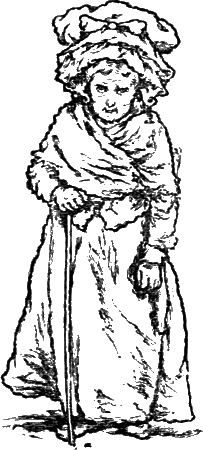
\includegraphics[height=2.8in]{fig-01.png}
\end{figure}

\pagebreak
This is the shoe.\\
And this is the dame\\
Without a name,\\
\textsc{Who Lived in the Shoe}.
\bigskip
\bigskip

\begin{figure}[H]
\centering
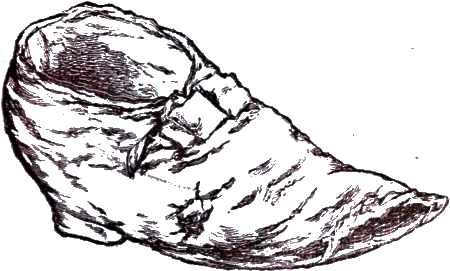
\includegraphics[height=2.8in]{fig-02.png}
\end{figure}

\pagebreak
These are the children, quite a score—--\\
Perhaps one less, perhaps one more—--\\
Who worried the dame without a name,\\
\textsc{Who Lived in the Shoe}.
\bigskip
\bigskip

\begin{figure}[H]
\centering
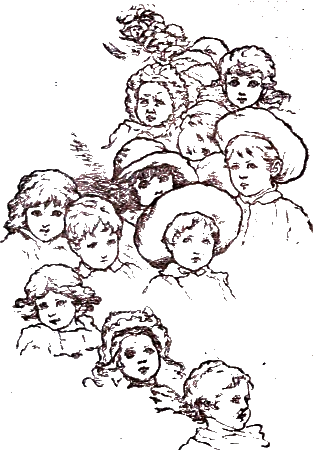
\includegraphics[height=2.8in]{fig-03}
\end{figure}

\pagebreak
This is the broth so weak and thin,\\
With never a bit of bread therein,\\
Made for the children, quite a score---\\
Perhaps one less, perhaps one more---\\
Who worried the dame without a name,\\
\textsc{Who Lived in the Shoe}.
\bigskip
\bigskip

\begin{figure}[H]
\centering
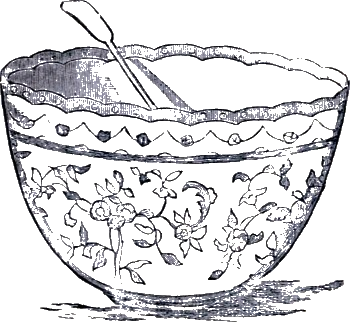
\includegraphics[height=2.8in]{fig-04}
\end{figure}

\pagebreak
This is the stick so long and thick,\\
That followed the broth so weak and thin,\\
With never a bit of bread therein,\\
Made for the children, quite a score---\\
Perhaps one less, perhaps one more---\\
Who worried the dame without a name,\\
\textsc{Who Lived in the Shoe}.
\bigskip
\bigskip

\begin{figure}[H]
\centering
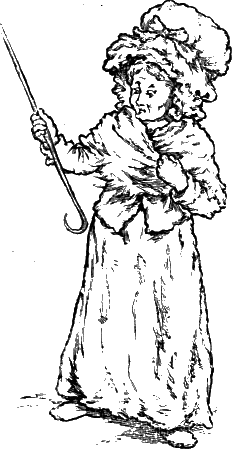
\includegraphics[height=2.8in]{fig-05}
\end{figure}

\pagebreak
This is the bed within the shoe,\\
That the children got in, two by two,\\
Urged by the stick so long and thick,\\
That followed the broth so weak and thin,\\
With never a bit of bread therein,\\
Made for the children, quite a score---\\
Perhaps one less, perhaps one more---\\
Who worried the dame without a name,\\
\textsc{Who Lived in the Shoe}.
\bigskip
\bigskip

\begin{figure}[H]
\centering
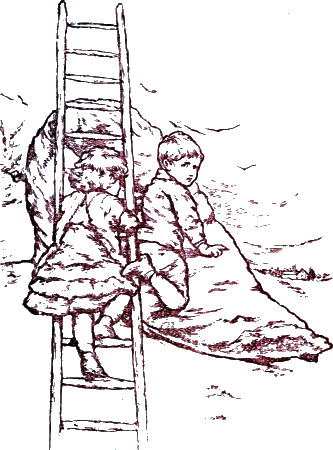
\includegraphics[height=2.8in]{fig-06}
\end{figure}

\pagebreak
And this is the end of a tale that is true,\\
Of a wonderful bed in a wonderful shoe,\\
That the children got in, two by two,\\
Urged by the stick so long and thick,\\
That followed the broth so weak and thin,\\
With never a bit of bread therein,\\
Made for the children, quite a score---\\
Perhaps one less, perhaps one more---\\
Who worried the dame without a name,\\
\textsc{Who Lived in the Shoe}.

\begin{figure}[H]
\centering
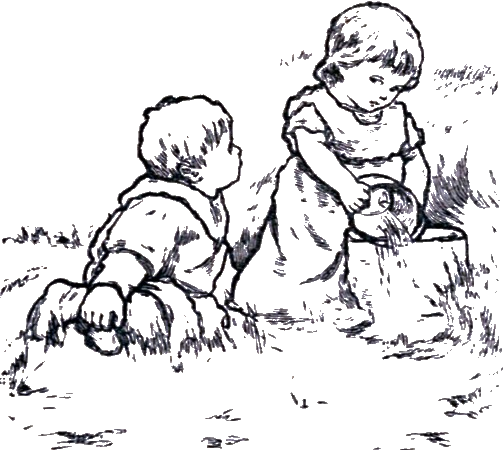
\includegraphics[height=2.6in]{fig-07}
\end{figure}

\ornamento

\end{document}
